\let\negmedspace\undefined
\let\negthickspace\undefined
\documentclass[journal,12pt,onecolumn,article]{IEEEtran}
\usepackage{cite}
\usepackage{color,soul}
\usepackage{amsmath,amssymb,amsfonts,amsthm}
\usepackage{algorithmic}
\usepackage{graphicx}
\usepackage{textcomp}
\usepackage{xcolor}
\usepackage{subcaption}
\usepackage{txfonts}
\usepackage{listings}
\usepackage{enumitem}
\usepackage{mathtools}
\usepackage{gensymb}
\usepackage{comment}
\usepackage[breaklinks=true]{hyperref}
\usepackage{tkz-euclide} 
\usepackage{listings}
\usepackage{multicol}
\usepackage{gvv}       
\usepackage[dvipsnames]{xcolor}
\def\inputGnumericTable{}                                
\usepackage[latin1]{inputenc}                            
\usepackage{color}                                       
\usepackage{array}                                       
\usepackage{longtable}                                   
\usepackage{calc}                                        
\usepackage{multirow}                                    
\usepackage{hhline}                                      
\usepackage{ifthen}                                      
\usepackage{lscape}
\usepackage{float}
\newtheorem{theorem}{Theorem}[section]
\newtheorem{problem}{Problem}
\newtheorem{proposition}{Proposition}[section]
\newtheorem{lemma}{Lemma}[section]
\newtheorem{corollary}[theorem]{Corollary}
\newtheorem{example}{Example}[section]
\newtheorem{definition}[problem]{Definition}
\newcommand{\BEQA}{\begin{eqnarray}}
\newcommand{\EEQA}{\end{eqnarray}}
\newcommand{\define}{\stackrel{\triangle}{=}}
\theoremstyle{remark}
\newtheorem{rem}{Remark}
\begin{document}
\bibliographystyle{IEEEtran}
\vspace{3cm}
\title{Gate-ASSIGNMENT-2}
\author{EE24BTECH11043 - Murra Rajesh Kumar Reddy}
\maketitle
\bigskip
\begin{enumerate}
	\item A single-stage gas turbine operates with an axial absolute flow at the entry and exit from the stage. The absolute flow angle at the nozzle exit is $70 \degree$. The turbine stage generates a specific work of $288 kJ/kg$ when operating with a mean blade speed of $440m/s$. The absolute velocity at the rotor entry is
		\begin{enumerate}
			\item $275.5 m/s$
			\item $551.5 m/s$
			\item $1103.0 m/s$
			\item $1654.5 m/s$
		\end{enumerate}
	\item An axial compressor operates such that is has an inlet and an exit total temparature of $300 K$ and $430 K$, respectiely. The isentropic efficency of the compressor is $85 \%$. If the ratio of specific heats is 1.4,then the total pressure ratio across the compressor is $\underline{\hspace{2cm}}$.
	\item The maximum value of coefficent of lift $\brak{C_1}$ for a 2D circular cylinder, provided at least one stagnation point lies on the cylinder surface, is predicted by the potential flow theory to be
		\begin{enumerate}
			\item $\pi/2$
			\item $\pi$
			\item $2\pi$
			\item $4\pi$
		\end{enumerate}
	\item The nozzle $\vec{AB}$, as shown below, leading to the test section of a low seed subsonic wind tunnel, has a contraction ratio of $10 : 1$. The pressure difference across the nozzle is maintained at $1000 N/m^2$ and the density of air is $1.23 kg/m^3$. Assuming one-dimensional, steady, inviscid flow, the velocity in the test section as measured at point $\vec{B}$ is $\underline{\hspace{1cm}} m/s$. \\
		\vspace{-75pt}
			\begin{figure}[H]
	\centering
				\begin{minipage}{0.75\textwidth}
	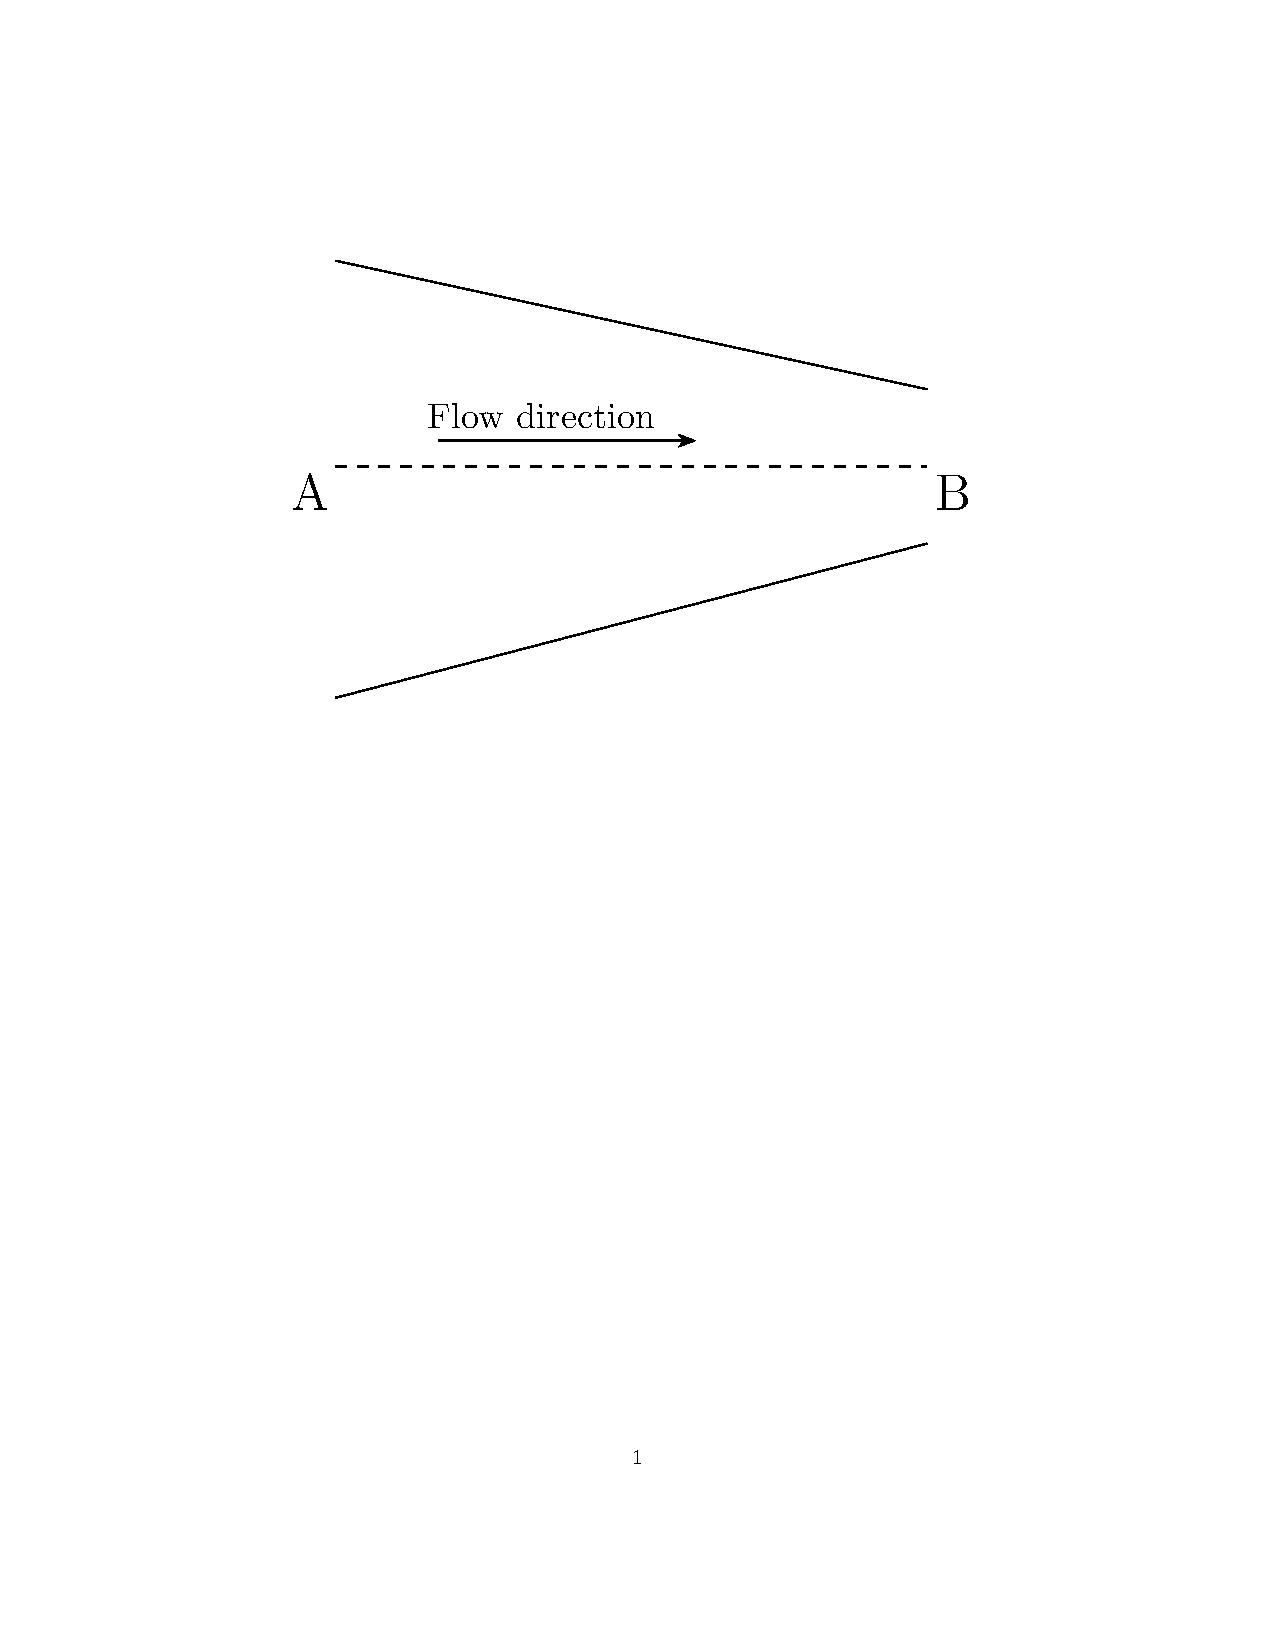
\includegraphics[width=0.7\linewidth]{fig/fig30/fig30.pdf}
			\end{minipage}
			\end{figure}
		\vspace{-180pt}

	\item The rate of change of moment coefficient with respect to the angle of attack, $\frac{dC_m}{d\alpha}$, at half chord point of a thin airfoil, as per approximations from the thin airfoil theory is
		\begin{enumerate}
			\item $\pi^2/16$
			\item $\pi^2/12$
			\item $\pi^2/8$
			\item $\pi/2$
		\end{enumerate}
	\item A gaseous mixture of air and fuel enters a constant area combustion chamber at a velocity of $100 m/s$ and at a static temparature of $300 K$. The heat release due to combustion is $100 J/kgK$. The total temparature of air-fuel mixture after combustion is $\underline{\hspace{1 cm}} K$.
	\item Consider 1-D, steady, inviscid, compressible flow through a convergent nozzle. The total temparature and total pressure are $T_o$, $P_o$ respectively. The flow through the nozzle is choked with a mass flow rate of $m_o$. If the total temparature is increased to $4T_o$, with total pressure remaining unchanged, then the mass flow rate through the nozzle
		\begin{enumerate}
			\item remains unchanged.
			\item becomes half of $\dot{m}_o$.
			\item becomes twice of $\dot{m}_o$.
			\item becomes four times of $\dot{m}_o$.
		\end{enumerate}
	\item Consider a second order linear ordinary differential equation $\frac{d^2y}{dx^2}-4\frac{dy}{dx}+4y=0$, with the boundary conditions $y\brak{0};\frac{dy}{dx}\bigg|_{x=0}=1$. The value of $y$ at $x=1$ is
		\begin{enumerate}
			\item $0$
			\item $1$
			\item $e$
			\item $e^2$
		\end{enumerate}
	\item Consider the following system of lineal equatins: \\
		$2x-y+z=1$ \\
		$3x-3y+4z=6$ \\
		$x-2y+3z=4$ \\
		This system of linear equation has
		\begin{enumerate}
			\item no solution.
			\item one solution.
			\item two solutions.
			\item three solutions.
		\end{enumerate}
	\item A bar made of linear elastic isotropic material is fixed at one end and subjected to an axial force of $1 kN$ at the other end. The cross-sectional area of the bar is $100 mm^2$, length is $100 mm$ and the Young's Modulus is $1 \times 10^5 N/mm^2$. The strain energy stored in the bar is $\underline{\hspace{1cm}} Nmm$.
	\item A cantilever beam-spring system is shown in the figure, The beam is made with a material of Young's modulus $1 \times 10^5 N/mm^2$ and geometry such that its moment of inertia is $100 mm^4$ and length l=100 mm. It is supported by a spring of stiffness $K=30 N/mm$ and subjected to a load of $P=100N$ at the point '$\vec{B}$'. The deflection at the point '$\vec{B}$' due to the load P is $\underline{\hspace{1 cm}}mm$.
		\vspace{-66pt}	
		\begin{figure}[H]
	\centering
				\begin{minipage}{0.71\textwidth}
	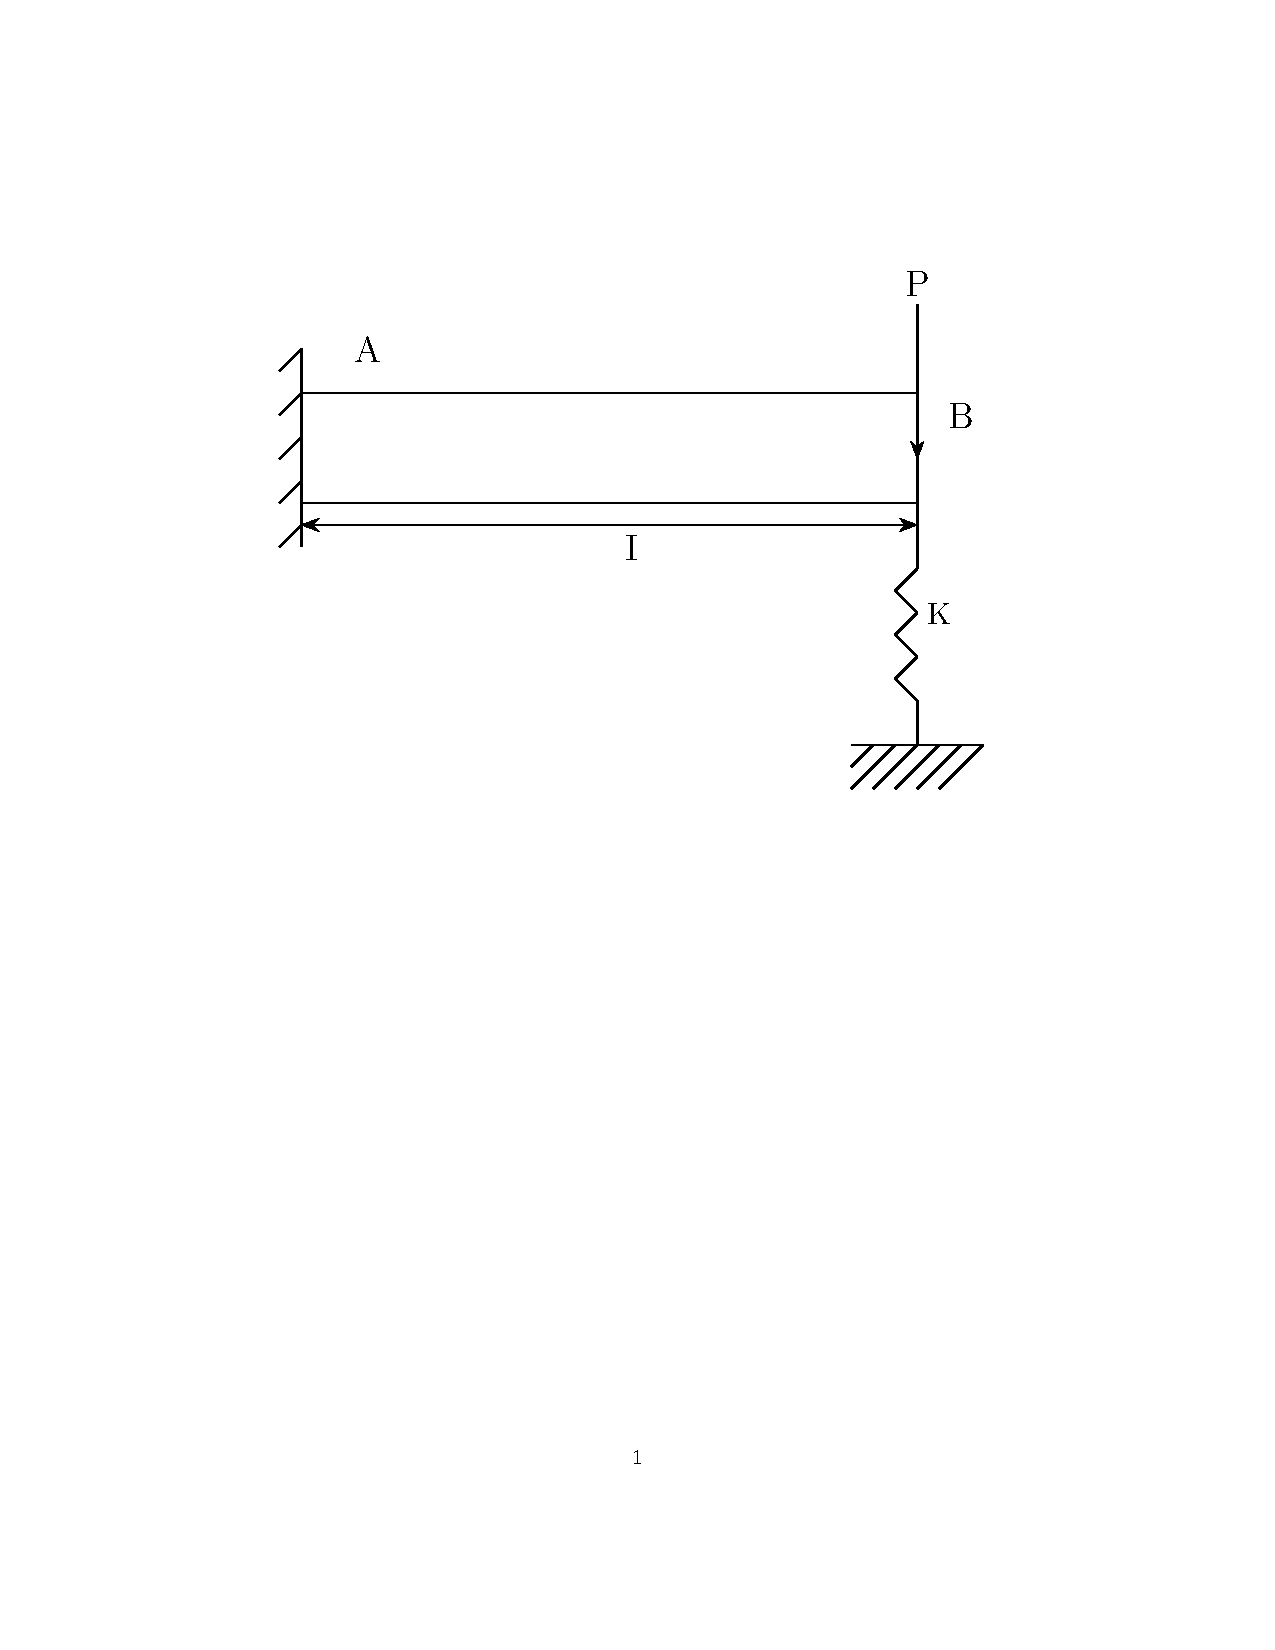
\includegraphics[width=0.7\linewidth]{fig/fig38/fig38.pdf}
				\end{minipage}
\end{figure}
\vspace{-60pt}
	\item Determne the correctness or otherwise of the following statements, $\sbrak{a}$ and $\sbrak{r}$, \\
		$\sbrak{a}$: Ribs, used in airplane wings, increase the column buckling strength of the longitudinal stiffners. \\
		$\sbrak{r}$: Ribs distribute concentrated loads into the structure and redistribute stresses around discontinuities.
		\begin{enumerate}
			\item Both $\sbrak{a}$ and $\brak{r}$ are true and $\sbrak{r}$ is the correct reason for $\sbrak{a}$
			\item Both $\sbrak{a}$ and $\sbrak{r}$ are ture but $\sbrak{r}$ is not the correct reason for $\sbrak{a}$
			\item Both $\sbrak{a}$ and $\sbrak{r}$ are false
			\item $\sbrak{a}$ is true but $\sbrak{r}$ is false
		\end{enumerate}
\end{enumerate}
\end{document}


